\documentclass[12pt]{article}
\begin{document}
\title{An efficient deep memory algorithm for computing fractional order operators}
\author{
Steven Dorsher and Gary W. Bohannan
}
\date{\today}

\maketitle

\begin{abstract}
This paper outlines a method to achieve effective bandwidth of five or more decades in the approximation of a fractional order derivative. This constitutes an increase of two decades or more over current algorithms, such the Infinite Impulse Response (IIR) method based on continued fraction expansion, while demanding only slightly more computational steps and processor memory. 
\end{abstract}

\section{Introduction}

Interest in the application of the fractional calculus has been
growing at an ever increasing rate. Of long term and continued
interest is in the use of fractional order (FO) operators, such as
integrators and differentiators, in motion control
applications.~\cite{Luo:13} While wide bandwidth analog controllers
have been successfully demonstrated~\cite{Bohannan:08}, fractional
order analog circuit elements are not generally available and the
prototypes that have been demonstrated do not have the ability to be
retuned for a specific desired phase.~\cite{Monje:10}

Unfortunately, the existing techniques for digital approximation of FO
operators are limited in bandwidth to on the order of three and a half
decades of frequency response while nonlinear effects in motion
control systems can span five decades or more. This places a severe
constraint on the design and implementation of digital FO controllers,
i.e. how to set the sampling frequency to meet the high speed
requirements necessitated by the Nyquist sampling rate while at the
same time providing enough deep memory to get low offset
error. Additionally, the infinite impulse response type of
implementation cannot guarantee stability due to the limitations of
finite precision arithmetic. See e.g.~\cite{Chen:04a}.

Given the current necessity to implement FO controls in digital form,
it is desirable to obtain the most efficient algorithm to compute a
fractional order operator while maximizing the numerical stability of
the algorithm. Efficiency to be measured in both memory utilization
and number of computations per time step. This paper outlines a
computational method inspired by the Riemann-Liouville integral
definition and the Gr{\"u}nwald algorithm.~\cite{OldSpan:74} The
essential concept is the rescaling of time by successive accumulation
of older data into increasing size bins for deeper memory.



\paragraph{Outline\\}
We will first briefly describe the current state of the art in fractional order operator approximation and then describe a novel approach based on successive binning of older data.

\begin{itemize} 
\item Section~\ref{algorithmDefn} will contain algorithm definitions. 
\item Section~\ref{results} will contain:
	\begin{itemize}
	\item  the amplitude and phase response of these algorithms for a large and small number of bins in the partition. 
	\item  an analysis of the computational resources required for the larger versus the smaller number of bins in the partition.
	\end{itemize}
\end{itemize}


\section{Algorithm definitions}\label{algorithmDefn}

\subsection{Partitioning the Grunwald history into averaged bins}\label{algorithmDefn_avgShift}
{\bf ADD REFERENCES}

The technology most widely used today in digital fractional order
circuitry is the continued fraction expansion (CFE) approximation to
$s^\alpha$. Its benefits are that it was a flat phase response over
approximately two and a half decades in phase for a 9th order
expansion (10 registers of input signal memory). It would be desirable
to find an algorithm with an even broader flat phase frequency
bandwidth and with a comparably small amount of memory required. We
take the Grunwald algorithm as a starting point. As the signal history
retained in the Grunwald sum grows longer, the bandwidth of flat phase
response grows broader; however, the memory required also increases
with input signal history length. To reduce this memory requirement
and retain a long signal history, we propose partitioning the input
signal history into bins that are longer further into the past. The
value of the binned input signal is represented by the average value
of the input signal within that bin. The presence of short bins at
recent times maintains sensitivity to high frequencies, while the
inclusion of long bins at past times adds sensitivity to low
frequencies that would not usually be present in a Grunwald sum with
the same number of terms. (See Figure~\ref{fig:freqScaling}).

\begin{figure}
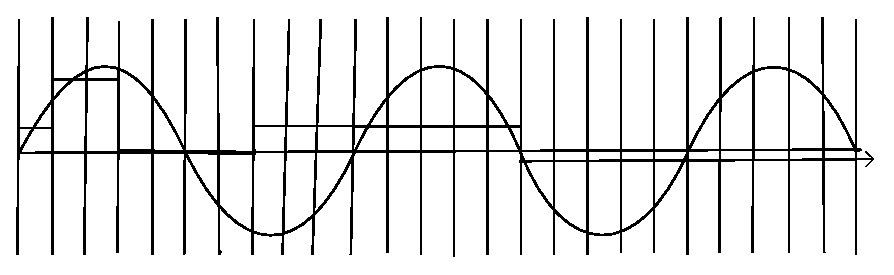
\includegraphics[width=3in]{sensitivityIsFreqDependent.eps}
\label{fig:freqScaling}
\caption{Let each division represent a single time step and each bar represent a bin, scaled such that the duration of a bin increases further back in time (toward the right). The value of the bin is the average of the input signal, the sine wave, at each point in time within that bin. There exists some oldest bin that responds sensitively to the input signal (in this figure, the second bin). For lower frequencies, that oldest bin moves to older times. This illustrates the sensitivity of short bins at recent times to high frequencies and long bins in the distant past to low frequencies.}
\end{figure}


\subsection{Modified Grunwald}

The Grunwald form of the fractional integral can be written

\begin{equation}
_0D^\alpha_tf(t) = \displaystyle \lim_{N\to\infty} \left(\frac{t}{N_t}\right)^{-\alpha}
\displaystyle\sum\limits_{j=0}^{N_t-1} w_{j}x_j
\label{simpleGrunwald}
\end{equation}
where $f(t)$ is the input signal at time $t$, the $j$th value of the
input signal history is $x_j=f\left(t-\frac{j\Delta t}{N_t}\right)$, and the
$j$th Grunwald weight is

\begin{equation}
w_{j} = \frac{\Gamma(j-\alpha)}{\Gamma(j+1)\Gamma(-\alpha)}.
\label{wj}
\end{equation}
To include more distant history at low computational cost, we modify
the Grunwald sum of Equation~\ref{simpleGrunwald} by partitioning its
history into $N_b$ bins. In each bin $k$, the input signal history
$x_j$ is represented by its average value over that bin, $X_k$.

Since we make the assumption that each value is well represented by
its average within a bin, we can define a value for the "bin
coefficient" by summing the Grunwald coefficients within that bin.

\begin{equation}
W_k = \displaystyle\sum\limits_{j=p_{k-1}+1}^{p_k} w_j
\label{eqn:sumWk}
\end{equation}

\noindent where $w_j$ is summed from the lowest index of the input data history within bin $k$ to the highest index $p_k$ within that bin. There is an additional factor that goes into $\bar{W}$ that will be discussed in Section~\ref{sec:shifting}. 

With these definitions, the modified Grunwald differ-integral can be written

\begin{equation}
_0D^\alpha_t f(t) = \displaystyle(\Delta t)^{-\alpha}\sum\limits_{k=0}^{N_b}\bar{W}_kX_k
\label{avgSimpleGrunwald}
\end{equation}
where $\Delta t$ is the interval between time samples.



\subsection{Updating the average history}
\label{sec:shifting}

When a new input data element is read, the history is updated. The new data element is shifted into the first bin through a weighted average. Since data elements represent time steps, they should be incompressible-- when one element is shifted into a bin, another virtual element should be shifted out of that bin if the bin is full. It shifts into the next bin, and pushes a virtual element out of that one, until a bin which is partially full or empty is reached. To update the average data stored in the bins, we take the weighted average obtained by adding one virtual element from the $(k-1)$th bin to the $b_k$ elements in the $k$th bin. This process is illustrated in Figure~\ref{fig:binShifting}.

\begin{figure}
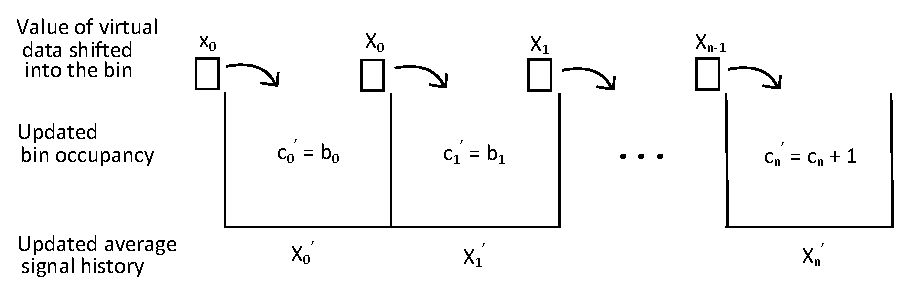
\includegraphics[width=4in]{binShifting.eps}
\label{fig:binShifting}
\caption{When the input data $x_0$ is read, virtual data elements with bin average values $X_k$ are shifted from the $k$th to the $(k+1)$th bin. The first $n-1$ bins are at capacity, but the $n$th bin gains one data point. The bin averages are updated to value $X_k^\prime$ through a weighted average.}
\end{figure}

During start-up, it will be necessary to consider bins that have some
set size $b_k$, but are not filled to that capacity. In that case, it
is the current occupation number $c_k$ of each bin that enters the
calculation. If the $k$th bin initially contains $c_k$ elements,
updating the history either leaves $c_k$ ($c_k\prime=c_k=b_k$) or
increments the number of elements in the bin such that $c_k\prime =
c_k + 1$ if the bin is not yet at capacity. Either way, the updated
average of the value of the $k$th bin, $X_k\prime$, is given by

\begin{equation}
X_k^\prime = \frac{c_k^\prime-1}{c_k^\prime}X_k + \frac{1}{c_k^\prime}X_{k-1}.
\label{eqn:updating}
\end{equation}
where $X_{-1}$ is taken to be $x_0$, the input data that has just been
read. 

During start-up, these partially full bins may also factor into
the Grunwald weights. To handle bins that are partially full, we
weight the binned Grunwald weights by the ratio of the bin occupation
number $c_k$ to its capacity $b_k$,

\begin{equation}
\bar{W}_k= \frac{c_k W_k}{b_k}.
\label{eqn:Wbar}
\end{equation} 











\section{Results}\label{results}

\subsection{Analysis of computational resources}
%
The computational efficiency of each algorithm concerns both the memory used by the algorithm and the number of computational steps required for the algorithm to execute, which is a measure of the speed. To characterize the operational efficiency of a digital fractor operating as a circuit element in real time, the quantities of interest are the memory or number of processor steps {/em per time step}.  

many of the variables defined in Section~\ref{algorithmDefn_avgShift} do not need to be stored. The Grunwald weights $w_i$ become temporary variables during initialization. The bin occupation numbers $c_k$ can be assumed to be equal to $b_k$ for a full bin (a fixed number at initialization) or zero for an empty bin. Only one bin along the partitioned history may be currently filling, and the filling progresses from low bin number to high bin number in numerical order. Therefore, there is no need to store the full array $c_k$. Instead, one may store the number of the bin that is filling, $k_{filling}$, and its current occupancy, $c_filling$, and from that information, fully recover the adjusted weight $\bar{W}_k$. There is also no advantage to storing $\bar{W}_k$, since it changes with each time step. With those considerations in mind, we enumerate the remaining variables in Table~\ref{tab:memory} to tabulate a total memory requirement for the Average-Shift algorithm.


\begin{table}[h]
\begin{tabular}{llll}
\hline
Variable& Definition & Size& Stages \\
\hline
$b_k$ & Bin capacity & $N_b$ &I, S, D \\
$W_k$ & Binned weights & $N_b$ &I, S, D \\
$X_k$ & Binned history & $N_b$ &I, S, D \\
$x_0$ & Current input data & 1 & S \\
$D_t^\alpha$ & Output differintegral & 1 & I, D\\
$\alpha$ &Order of differintegral &1 &I, D\\
$N_b$ &Number of bins &1 &I,S,D\\
$N_t$ &Number of time steps stored &1 & I\\
$\Delta t$ &Time step &1 &D\\
$w_i$ & Grunwald weight, temp variable & 1 & I\\
$k_{filling}$ & Currently filling bin & 1 & S, D\\
$c_{filling}$ & Occupancy of filling bin & 1 & S, D \\  
\hline
\hline
& Total w/o initialization &$3N_b+6$ &\\
 & Total & $3N_b+9$ &\\
\hline
\end{tabular}
\label{tab:memory}
\caption{Accounting for memory in the Average-Shift algorithm. I = Initialization, S = Shifting, D = Differintegration}
\end{table}

To calculate the number of computational steps required for initialization, we combine the cost of initializing relevant variables to zero with the cost of computing the binned weights, while we neglect the cost of initializing the shape of the partitioned history. This is because the choice of the number of elements per bin, $b_k$, may be application dependent and has a startup cost associated with it that is highly depended upon the functional form of $b_k$. $W_k$, $X_K$, $k_{filling}$, and $c_{filling}$ must initially be set to zero and $w_0$ must be set to one for a total of $2N_b+3$ computational steps. To compute $W_k$, we rely on the recursion formula for the Grunwald weights

\begin{equation}
w_j = \frac{j-1-\alpha}{j}w_{j-1}.
\label{eqn:GrunwaldRecursion}
\end{equation}

ELIMINATE $H_{max}$

FIX SPEED, INITIALIZATION

\noindent There are four arithmetic steps per recursion, plus one count step to increment $j$. Since the initial value $w_0=1$ has been set exactly, there are $H_{max}-1$ recursive steps to get to the last of the $H_{max}$ Grunwald weights at the end of the $N_b$ bins. This produces a total of $5H_{max}-5$ computational steps to calculate the Grunwald weights so far. These Grunwald weights are not stored, but rather, they are summed together into binned weights as the computation progresses. Between the $N_b$ bins, there are between zero and $H_{max}-1$ sums taken depending on the bin structure of the partitioned history. Totalling the number of computational steps, there are between $2N_b+5H_{max}-2$ and $2N_b+6H_{max}-3$ computational steps taken during the initialization process, neglecting the actual operation of partitioning the history into bins. Initialization speed depends more strongly on the maximum signal memory depth of the partitioned history than on the number of bins in the partition. 

During the shifting phase, where a new data point is read in from the outside world and added to the partitioned history, there are two possible cases: the binned history may already be full, or it may still be filling. There are six arithmetic steps required to evaluate Equation~\ref{}. It is only necessary to evaluate this expression for $k\le k_{filling}$, for a total of $6k_{filling}$ steps so far. For $k<k_{filling}$, $c_k'=b_k$ so no additional calculation is necessary; however, it is necessary to test that it falls within this region with an if statement. That adds $k_{filling}-1$ additional steps. On the other hand, for $k=k_{filling}$, $c_k$ must be incremented to obtain $c_k'$, adding two additional steps. Incrementing $k_{filling}$ if $c_{filling}=b_{k,{filling}}$ adds another two steps. Checking to be sure that $k<N_b$ at all times adds another step. Adding all these computational steps together, we obtain the total of $7k_{filling}+4$ computational steps required to shift a new data element into the binned history. From this, we see that partially filled binned histories operate more quickly than filled ones, and the steady-state speed of a filled history scales its number of bins.

Likewise, integration has two cases, depending whether or not the history has been filled.  

\begin{table}
\begin{tabular}
\hline
Stage& Computational Steps\\
Initialization & $5H_{Max}+2N_b-2$ to $6H_{max}+2N_b-3$\\
Shifting & 7k_{filling}+4 \rightarrow 7N_b+4$\\

\hline
\hline
Total & \\
\hline
\end{tabular}
\label{tab:speed}
\caption{Number of computational steps required for Average-Shift algorithm.}
\end{table}

\section{Conclusions}\label{conclusions}

\bibliographystyle{unsrt}
\bibliography{BohannanFull}

\end{document}

